\chapter{Joint Inversion}\label{Chp:cook:joint inversion}


Interpretation of a joint inversion 3D model of gravity and magnetic data could solve a big problem of exploration geophysics. Traditionally inversion of magnetic and gravity data provide a 3D physical rock property model separately, However in this section a new package is presented to provide a joint model of density and magnetic susceptibility which undertake an apparent discrepancy in terms of geolophysical approach. This package is based on geological smooth model in density and magnetic susceptibility variations.\\

\textbf{Input File} \\


A small part of sample of inversion_gravmag_3d:\\
\begin{verbatim}
depth_offset = 10. * U.km
n_humps_h = 3
n_humps_v = 1
n_humpsm_h =2
n_humpsm_v =1
mu = 100.
n_cells_in_data = 30
latitude = -28.5
l_data = 100. * U.km
l_pad = 40. * U.km
THICKNESS = 20. * U.km
l_air = 6. * U.km
\end{verbatim}

inversion_gravmag file consist many options to implement which control how joint inversion is performed such as padding area, depth , MU factor,\ldots. which in previous section was explaind in deatails. just some items are fixed for joint inversion such as mu.\\

\begin{description} 	
\item[latitude]this is refered to the area of gathering data sets to calculate the main reference magnetic field. which is selected -28 for east Australia.


\item[mu]It is defined in accordance with the noise of data it is 100 for this section.

\end{description}

\textbf{Output File}\\


\textbf{Reference}\\

this is a 3D model as an example with three different density humps and two different susceptibility humps in horizon. this made nine density humps and four susceptibility humps. Two first image show the reference synthetic datasets and two last images indicate result after joint inversion in two both magnetic and gravity 
 
\begin{verbatim}
n_humps_h = 3
n_humps_v = 1
n_humpsm_h =2
n_humpsm_v =1
mu=100
\end{verbatim}

\begin{figure}
\centering
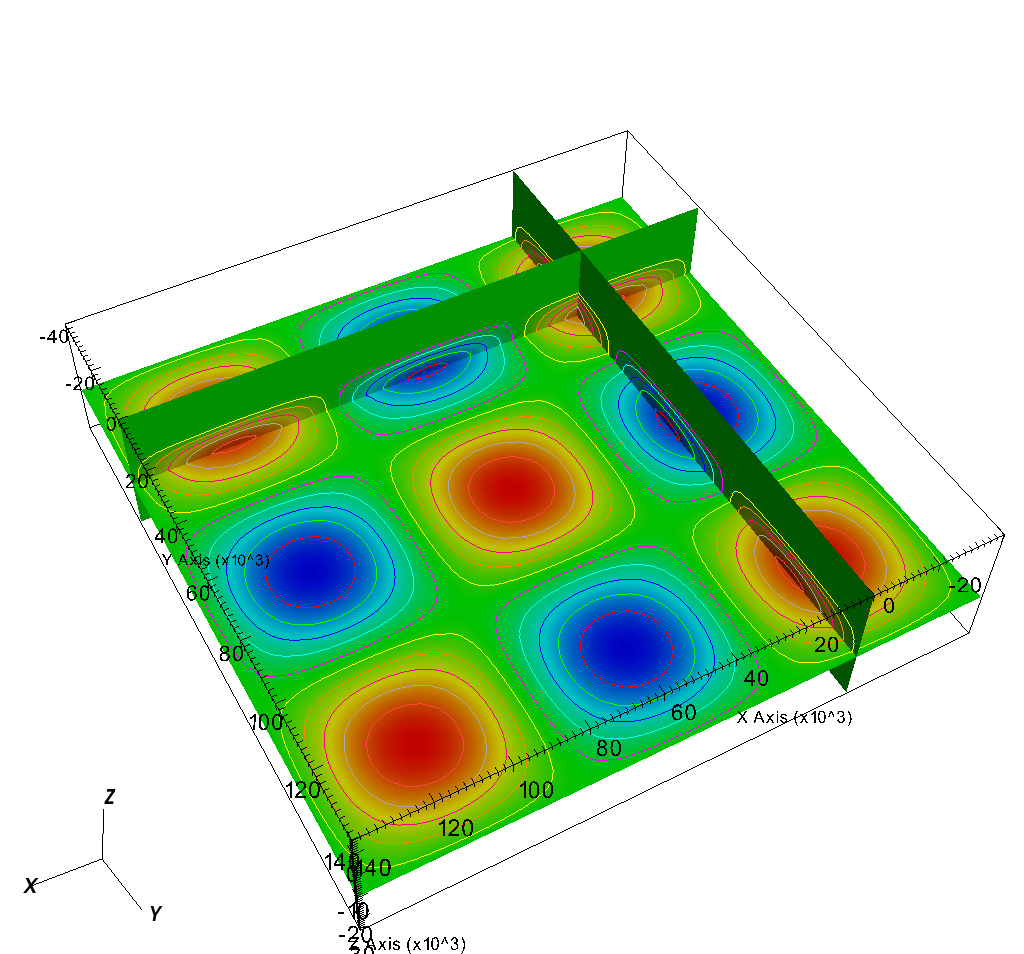
\includegraphics[width=\textwidth]{joint3D4mag6grav-gref.png}
\caption{3D reference density model}

\end{figure}



\begin{figure}
\centering
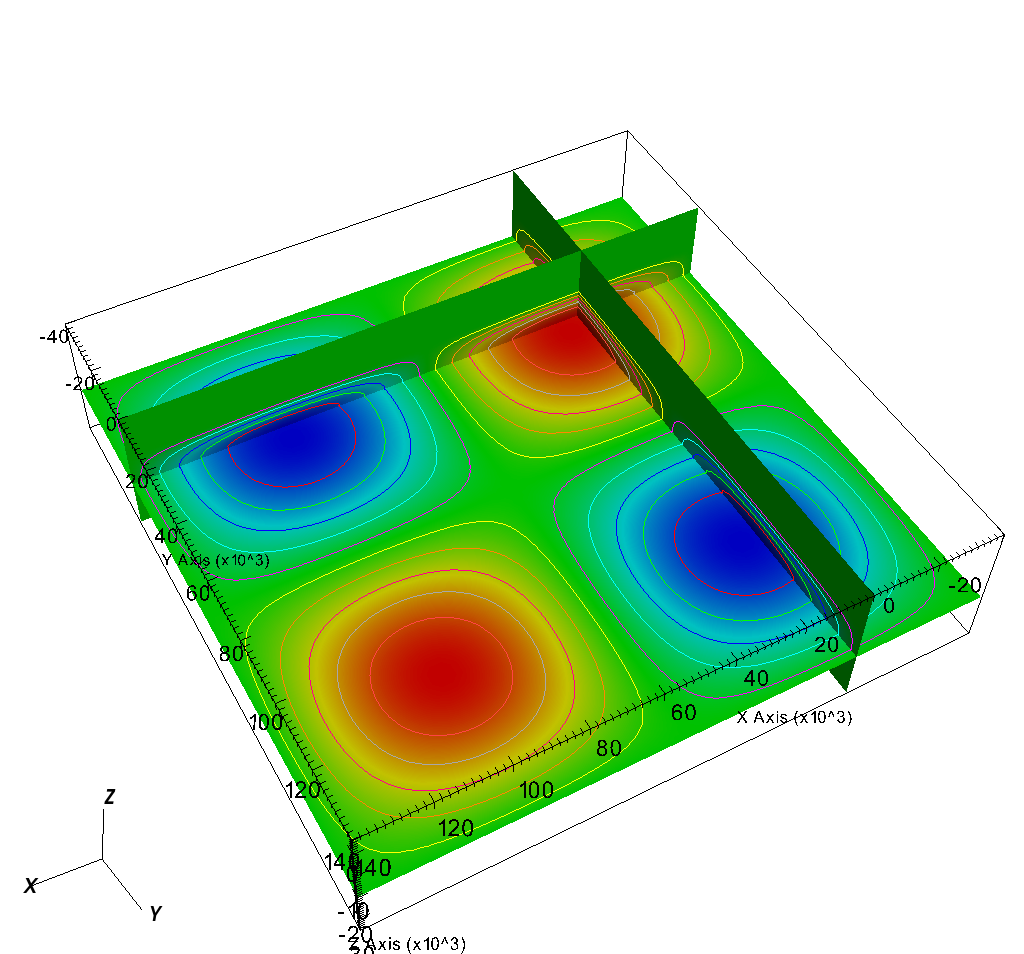
\includegraphics[width=\textwidth]{joint3D4mag6grav-mref.png}
\caption{3D reference susceptibility model}

\end{figure}


\begin{figure}
\centering
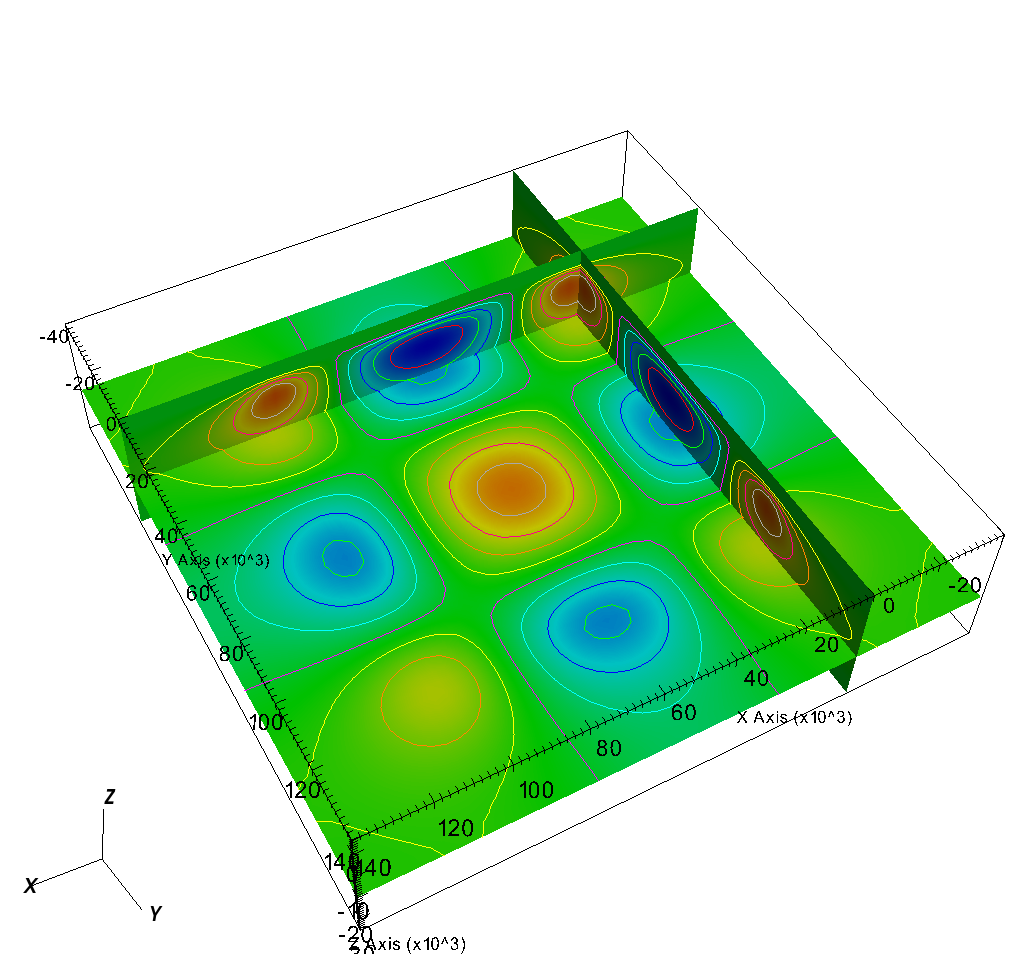
\includegraphics[width=\textwidth]{joint3D4mag6grav-g.png}
\caption{3D result density model}

\end{figure}


\begin{figure}
\centering
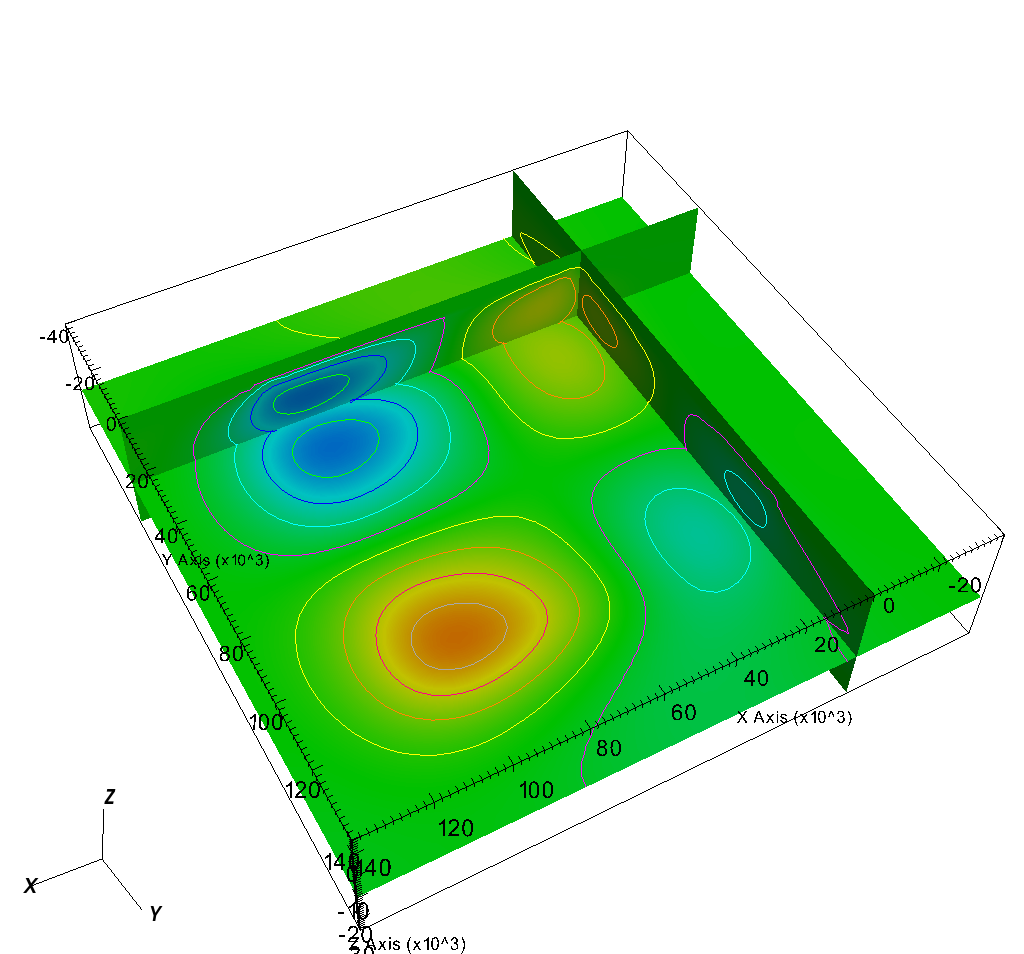
\includegraphics[width=\textwidth]{joint3D4mag6grav-m.png}
\caption{3D result magnetic model}

\end{figure}

